
%(BEGIN_QUESTION)
% Copyright 2008, Tony R. Kuphaldt, released under the Creative Commons Attribution License (v 1.0)
% This means you may do almost anything with this work of mine, so long as you give me proper credit

En {\it sentrifugalpumpe} virker ved å rotere en skive med radiale skovler kalt et ``impeller,'' som slynger væske utover fra sentrum av skiven til kanten av skiven. Denne kinetiske energien som tilføres væsken, omdannes til potensiell energi i form av trykk når væskemolekylene treffer innerveggen i pumpehuset:

$$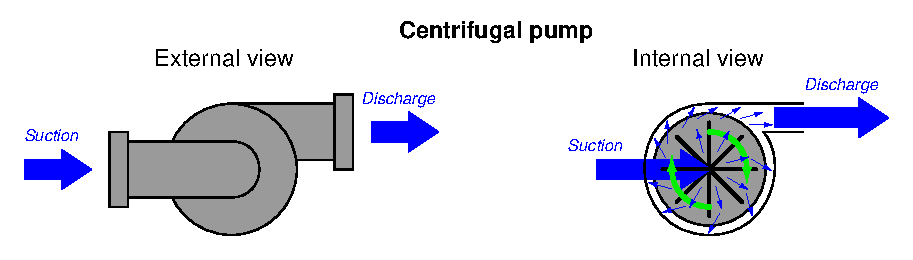
\includegraphics[width=15.5cm]{i01407x03.eps}$$

Ytelsen til en sentrifugalpumpe uttrykkes ofte i en spesialgraf kalt en {\it pumpekurve}. En typisk pumpekurve for en sentrifugalpumpe ser slik ut:

$$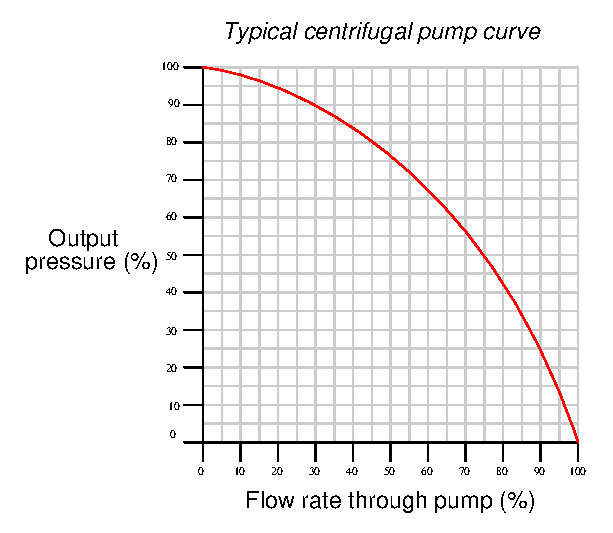
\includegraphics[width=15.5cm]{i01407x01.eps}$$

Undersøk denne pumpekurven, og forklar med egne ord hva den forteller oss om pumpens ytelsesoppførsel.

\vskip 20pt \vbox{\hrule \hbox{\strut \vrule{} {\bf Forslag til sokratisk diskusjon} \vrule} \hrule}

\begin{itemize}
\item{} En måte å beskrive virkemåten til en sentrifugalpumpe på, er å si at den genererer utløpstrykk ved å konvertere kinetisk energi til potensiell energi. Utdyp denne påstanden, og forklar nøyaktig hvor og hvordan kinetisk energi blir konvertert til potensiell energi. Hint: Dette er enklere å svare på dersom du ser på ``grensetilfellet'' med maksimalt utløpstrykk i pumpekurven, der strømningen er null og trykket er maksimalt.
\item{} Med utgangspunkt i energiomdanningen mellom kinetisk og potensiell form, forklar {\it hvorfor} utløpstrykket for en sentrifugalpumpe faller når strømningsraten øker.
\item{} Den viste pumpekurven forutsetter konstant rotasjonshastighet på pumpehjulet. Hvordan ville pumpekurven endret seg dersom pumpen roterte saktere?
\end{itemize}

\underbar{file i01407}
%(END_QUESTION)





%(BEGIN_ANSWER)

Denne grafen viser sammenhengen mellom trykkutgang og væskestrømningsrate for en sentrifugalpumpe som går med konstant rotasjonshastighet.
 
%(END_ANSWER)





%(BEGIN_NOTES)

En {\it pumpekurve} er en graf over trykkutgang versus væskestrømningsrate for en sentrifugalpumpe ved konstant rotasjonshastighet. Pumpekurver er avgjørende for å beregne presise trykk- og strømningsverdier i væskepumpesystemer.

\vskip 10pt

Sentrifugalpumper er i sin natur {\it inertielle}. De virker ved å tilføre væskemolekylene kinetisk energi, ikke ved å flytte faste væskevolumer per omdreining slik en fortrengningspumpe gjør (per definisjon). En måte å se forskjellen på er å spørre seg om væske kan strømme fritt gjennom pumpemekanismen ved hjelp av en ekstern trykkilde dersom pumpeakselen setter seg fast og blir stående. For en ekte fortrengningspumpe vil væskestrømmen blokkeres: ingen akselbevegelse betyr at væskevolum {\it ikke kan} passere gjennom pumpen.

\vskip 10pt

En fortrengningspumpe som roterer med konstant hastighet, vil pumpe en konstant strømningsrate uavhengig av trykk. Derfor er den ideelle pumpekurven for en fortrengningspumpe en vertikal linje:

$$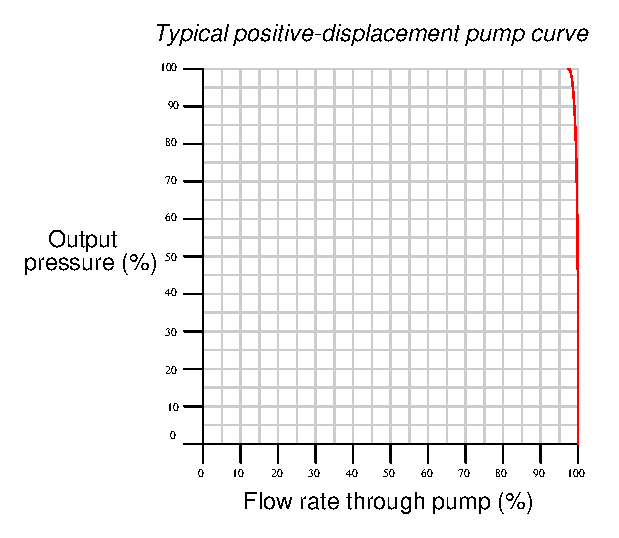
\includegraphics[width=15.5cm]{i01407x02.eps}$$

Den reelle pumpekurven for en fortrengningspumpe vil bøye litt av øverst (mot venstre) på grunn av internlekkasje når trykket øker.

\vfil \eject

\noindent
{\bf Forberedelsesquiz:}

En {\it pumpekurve} beskriver:

\begin{itemize}
\item{} Korrekt bøyeradius for rørbend før og etter en pumpe
\vskip 5pt 
\item{} Krummingen i strømningsbanen når væske går inn i pumpehuset
\vskip 5pt 
\item{} Trykk- versus strømningskarakteristikkene til en pumpe
\vskip 5pt 
\item{} Mengden væsketurbulens inne i en pumpe ved ulike hastigheter
\vskip 5pt 
\item{} Maksimal væsketetthet en pumpe kan håndtere
\vskip 5pt 
\item{} Pumpens effektbehov ved ulike væsketettheter
\end{itemize}


%INDEX% Final Control Elements, pump: pressure/flow curve
%INDEX% Machine, centrifugal pump

%(END_NOTES)

